% Options for packages loaded elsewhere
\PassOptionsToPackage{unicode}{hyperref}
\PassOptionsToPackage{hyphens}{url}
\PassOptionsToPackage{dvipsnames,svgnames,x11names}{xcolor}
%
\documentclass[
  letterpaper,
  DIV=11,
  numbers=noendperiod]{scrartcl}

\usepackage{amsmath,amssymb}
\usepackage{lmodern}
\usepackage{iftex}
\ifPDFTeX
  \usepackage[T1]{fontenc}
  \usepackage[utf8]{inputenc}
  \usepackage{textcomp} % provide euro and other symbols
\else % if luatex or xetex
  \usepackage{unicode-math}
  \defaultfontfeatures{Scale=MatchLowercase}
  \defaultfontfeatures[\rmfamily]{Ligatures=TeX,Scale=1}
\fi
% Use upquote if available, for straight quotes in verbatim environments
\IfFileExists{upquote.sty}{\usepackage{upquote}}{}
\IfFileExists{microtype.sty}{% use microtype if available
  \usepackage[]{microtype}
  \UseMicrotypeSet[protrusion]{basicmath} % disable protrusion for tt fonts
}{}
\makeatletter
\@ifundefined{KOMAClassName}{% if non-KOMA class
  \IfFileExists{parskip.sty}{%
    \usepackage{parskip}
  }{% else
    \setlength{\parindent}{0pt}
    \setlength{\parskip}{6pt plus 2pt minus 1pt}}
}{% if KOMA class
  \KOMAoptions{parskip=half}}
\makeatother
\usepackage{xcolor}
\setlength{\emergencystretch}{3em} % prevent overfull lines
\setcounter{secnumdepth}{-\maxdimen} % remove section numbering
% Make \paragraph and \subparagraph free-standing
\ifx\paragraph\undefined\else
  \let\oldparagraph\paragraph
  \renewcommand{\paragraph}[1]{\oldparagraph{#1}\mbox{}}
\fi
\ifx\subparagraph\undefined\else
  \let\oldsubparagraph\subparagraph
  \renewcommand{\subparagraph}[1]{\oldsubparagraph{#1}\mbox{}}
\fi

\usepackage{color}
\usepackage{fancyvrb}
\newcommand{\VerbBar}{|}
\newcommand{\VERB}{\Verb[commandchars=\\\{\}]}
\DefineVerbatimEnvironment{Highlighting}{Verbatim}{commandchars=\\\{\}}
% Add ',fontsize=\small' for more characters per line
\usepackage{framed}
\definecolor{shadecolor}{RGB}{241,243,245}
\newenvironment{Shaded}{\begin{snugshade}}{\end{snugshade}}
\newcommand{\AlertTok}[1]{\textcolor[rgb]{0.68,0.00,0.00}{#1}}
\newcommand{\AnnotationTok}[1]{\textcolor[rgb]{0.37,0.37,0.37}{#1}}
\newcommand{\AttributeTok}[1]{\textcolor[rgb]{0.40,0.45,0.13}{#1}}
\newcommand{\BaseNTok}[1]{\textcolor[rgb]{0.68,0.00,0.00}{#1}}
\newcommand{\BuiltInTok}[1]{\textcolor[rgb]{0.00,0.23,0.31}{#1}}
\newcommand{\CharTok}[1]{\textcolor[rgb]{0.13,0.47,0.30}{#1}}
\newcommand{\CommentTok}[1]{\textcolor[rgb]{0.37,0.37,0.37}{#1}}
\newcommand{\CommentVarTok}[1]{\textcolor[rgb]{0.37,0.37,0.37}{\textit{#1}}}
\newcommand{\ConstantTok}[1]{\textcolor[rgb]{0.56,0.35,0.01}{#1}}
\newcommand{\ControlFlowTok}[1]{\textcolor[rgb]{0.00,0.23,0.31}{#1}}
\newcommand{\DataTypeTok}[1]{\textcolor[rgb]{0.68,0.00,0.00}{#1}}
\newcommand{\DecValTok}[1]{\textcolor[rgb]{0.68,0.00,0.00}{#1}}
\newcommand{\DocumentationTok}[1]{\textcolor[rgb]{0.37,0.37,0.37}{\textit{#1}}}
\newcommand{\ErrorTok}[1]{\textcolor[rgb]{0.68,0.00,0.00}{#1}}
\newcommand{\ExtensionTok}[1]{\textcolor[rgb]{0.00,0.23,0.31}{#1}}
\newcommand{\FloatTok}[1]{\textcolor[rgb]{0.68,0.00,0.00}{#1}}
\newcommand{\FunctionTok}[1]{\textcolor[rgb]{0.28,0.35,0.67}{#1}}
\newcommand{\ImportTok}[1]{\textcolor[rgb]{0.00,0.46,0.62}{#1}}
\newcommand{\InformationTok}[1]{\textcolor[rgb]{0.37,0.37,0.37}{#1}}
\newcommand{\KeywordTok}[1]{\textcolor[rgb]{0.00,0.23,0.31}{#1}}
\newcommand{\NormalTok}[1]{\textcolor[rgb]{0.00,0.23,0.31}{#1}}
\newcommand{\OperatorTok}[1]{\textcolor[rgb]{0.37,0.37,0.37}{#1}}
\newcommand{\OtherTok}[1]{\textcolor[rgb]{0.00,0.23,0.31}{#1}}
\newcommand{\PreprocessorTok}[1]{\textcolor[rgb]{0.68,0.00,0.00}{#1}}
\newcommand{\RegionMarkerTok}[1]{\textcolor[rgb]{0.00,0.23,0.31}{#1}}
\newcommand{\SpecialCharTok}[1]{\textcolor[rgb]{0.37,0.37,0.37}{#1}}
\newcommand{\SpecialStringTok}[1]{\textcolor[rgb]{0.13,0.47,0.30}{#1}}
\newcommand{\StringTok}[1]{\textcolor[rgb]{0.13,0.47,0.30}{#1}}
\newcommand{\VariableTok}[1]{\textcolor[rgb]{0.07,0.07,0.07}{#1}}
\newcommand{\VerbatimStringTok}[1]{\textcolor[rgb]{0.13,0.47,0.30}{#1}}
\newcommand{\WarningTok}[1]{\textcolor[rgb]{0.37,0.37,0.37}{\textit{#1}}}

\providecommand{\tightlist}{%
  \setlength{\itemsep}{0pt}\setlength{\parskip}{0pt}}\usepackage{longtable,booktabs,array}
\usepackage{calc} % for calculating minipage widths
% Correct order of tables after \paragraph or \subparagraph
\usepackage{etoolbox}
\makeatletter
\patchcmd\longtable{\par}{\if@noskipsec\mbox{}\fi\par}{}{}
\makeatother
% Allow footnotes in longtable head/foot
\IfFileExists{footnotehyper.sty}{\usepackage{footnotehyper}}{\usepackage{footnote}}
\makesavenoteenv{longtable}
\usepackage{graphicx}
\makeatletter
\def\maxwidth{\ifdim\Gin@nat@width>\linewidth\linewidth\else\Gin@nat@width\fi}
\def\maxheight{\ifdim\Gin@nat@height>\textheight\textheight\else\Gin@nat@height\fi}
\makeatother
% Scale images if necessary, so that they will not overflow the page
% margins by default, and it is still possible to overwrite the defaults
% using explicit options in \includegraphics[width, height, ...]{}
\setkeys{Gin}{width=\maxwidth,height=\maxheight,keepaspectratio}
% Set default figure placement to htbp
\makeatletter
\def\fps@figure{htbp}
\makeatother

\KOMAoption{captions}{tableheading}
\makeatletter
\makeatother
\makeatletter
\makeatother
\makeatletter
\@ifpackageloaded{caption}{}{\usepackage{caption}}
\AtBeginDocument{%
\ifdefined\contentsname
  \renewcommand*\contentsname{Table of contents}
\else
  \newcommand\contentsname{Table of contents}
\fi
\ifdefined\listfigurename
  \renewcommand*\listfigurename{List of Figures}
\else
  \newcommand\listfigurename{List of Figures}
\fi
\ifdefined\listtablename
  \renewcommand*\listtablename{List of Tables}
\else
  \newcommand\listtablename{List of Tables}
\fi
\ifdefined\figurename
  \renewcommand*\figurename{Figure}
\else
  \newcommand\figurename{Figure}
\fi
\ifdefined\tablename
  \renewcommand*\tablename{Table}
\else
  \newcommand\tablename{Table}
\fi
}
\@ifpackageloaded{float}{}{\usepackage{float}}
\floatstyle{ruled}
\@ifundefined{c@chapter}{\newfloat{codelisting}{h}{lop}}{\newfloat{codelisting}{h}{lop}[chapter]}
\floatname{codelisting}{Listing}
\newcommand*\listoflistings{\listof{codelisting}{List of Listings}}
\makeatother
\makeatletter
\@ifpackageloaded{caption}{}{\usepackage{caption}}
\@ifpackageloaded{subcaption}{}{\usepackage{subcaption}}
\makeatother
\makeatletter
\@ifpackageloaded{tcolorbox}{}{\usepackage[many]{tcolorbox}}
\makeatother
\makeatletter
\@ifundefined{shadecolor}{\definecolor{shadecolor}{rgb}{.97, .97, .97}}
\makeatother
\makeatletter
\makeatother
\ifLuaTeX
  \usepackage{selnolig}  % disable illegal ligatures
\fi
\IfFileExists{bookmark.sty}{\usepackage{bookmark}}{\usepackage{hyperref}}
\IfFileExists{xurl.sty}{\usepackage{xurl}}{} % add URL line breaks if available
\urlstyle{same} % disable monospaced font for URLs
\hypersetup{
  pdftitle={Introduccion\_al\_aprendizaje\_automatico},
  pdfauthor={Katherine\_Criollo\_y\_Victoria\_Peñafiel},
  colorlinks=true,
  linkcolor={blue},
  filecolor={Maroon},
  citecolor={Blue},
  urlcolor={Blue},
  pdfcreator={LaTeX via pandoc}}

\title{Introduccion\_al\_aprendizaje\_automatico}
\author{Katherine\_Criollo\_y\_Victoria\_Peñafiel}
\date{}

\begin{document}
\maketitle
\ifdefined\Shaded\renewenvironment{Shaded}{\begin{tcolorbox}[borderline west={3pt}{0pt}{shadecolor}, interior hidden, breakable, sharp corners, enhanced, boxrule=0pt, frame hidden]}{\end{tcolorbox}}\fi

\hypertarget{introducciuxf3n-al-aprendizaje-automuxe1tico}{%
\subsection{INTRODUCCIÓN AL APRENDIZAJE
AUTOMÁTICO}\label{introducciuxf3n-al-aprendizaje-automuxe1tico}}

Enseñar a una computadora es una tarea que se encuentra ligada a que
ella aprenda a jugar, responder preguntas triviales o que reflexione
sobre filosofía. Mientras que el aprendizaje automático se asemeja a
entrenar en algo a un empleado y no a criarlo desde que es un niño.
Después de esta breve introducción sobre el capítulo, en el mismo se
tratarán varios temas como: • Los orígenes y las aplicaciones prácticas
del aprendizaje automático • Cómo las computadoras definen y representan
el conocimiento • Los conceptos básicos que diferencian los enfoques del
aprendizaje automático

\hypertarget{los-oruxedgenes-y-las-aplicaciones-pruxe1cticas-del-aprendizaje-automuxe1tico}{%
\subsubsection{Los orígenes y las aplicaciones prácticas del aprendizaje
automático}\label{los-oruxedgenes-y-las-aplicaciones-pruxe1cticas-del-aprendizaje-automuxe1tico}}

Desde que un ser humano nace comienza a recibir e interpretar datos por
medio de sus sentidos, el cerebro procesa esta información en forma de
sonidos, olores, imágenes, entre otros y da una respuesta. Durante
muchos años los encargados de registrar y dar respuestas a distintos
datos y estadísticas eran los seres humanos, pero en la actualidad este
proceso se a vuelto autónomo y rápidos en donde una computadora realiza
todo el proceso y los guarda en bases de datos. La creación de sensores
a contribuido a que se pueda aumentar la calidad y la cantidad de datos
registrados y procesados, lo que ha facilitado que gobiernos, empresas e
industrias obtengan cualquier tipo de datos de manera más rápida y
fácil. En la actualidad nos encontramos en la denominada era Big Data,
aunque siempre han existido gran cantidad de datos, lo que caracteriza a
esta era es la accesibilidad que tiene cada persona para interactuar y
usar los registros de datos. El aprendizaje automático es un campo que
tiene el objetivo de desarrollar algoritmos de trasformación de datos a
acciones, además que la minería de datos se basa en recolectar distintas
bases y registros de datos y convertirlos en información novedosa, estos
dos campos, aunque se complementan, tiene la diferencia que el primero
se enfoca solo en realiza una tarea conocida, mientras que el otro busca
pepitas de información ocultas.

\hypertarget{usos-y-abusos-del-aprendizaje-automuxe1tico}{%
\subsubsection{Usos y abusos del aprendizaje
automático}\label{usos-y-abusos-del-aprendizaje-automuxe1tico}}

El aprendizaje automático tiene como objetivo dar sentido o respuesta a
los datos complejos, esta misión es aplicable a distintos campos y se
utiliza en distintos casos:

• Predecir los resultados de las elecciones.

• Identificar y filtrar los mensajes de spam del correo electrónico.

• Prever la actividad delictiva.

• Automatizar las señales de tráfico de acuerdo con las condiciones de
la carretera.

• Producir estimaciones financieras de tormentas y desastres naturales.

El procedimiento del aprendizaje automático genera algoritmos que
identifiquen distintos patrones para cumplir con una acción especifica,
un ejemplo de esto es donde un minorista utilizó el aprendizaje
automático para identificar a mujeres embarazadas para enviarles cupones
específicos, basados en los patrones que ellas seguían como las compras
de vitaminas prenatales, lociones y toallitas. El minorista tenía el
objetivo de que las futuras madres fueran clientes leales que compraran
artículos rentables como pañales, fórmula y juguetes. Esto es una
práctica que normalmente los minoristas realizan en donde ellos acceden
a las transacciones de sus clientes y utilizando el método del
aprendizaje automático generan publicidad, promociones, entre otros.
Este método también utiliza los sitios web donde ellos utilizan los
datos de navegación, para conocer los intereses de los usuarios y mandar
anuncios y recomendaciones. Con este método se sugiere que se tome en
cuenta las implicaciones éticas del uso de datos de los usuarios.

\hypertarget{consideraciones-uxe9ticas}{%
\subsubsection{Consideraciones éticas}\label{consideraciones-uxe9ticas}}

El aprendizaje automático es un campo joven el cual está en constante
evolución, lo que provoca que legalmente y socialmente su desarrollo sea
incierto, por tal motivo el acceder a distintos datos tiene que ser bajo
mucha precaución para no incurrir en la violación de ninguna ley,
abusando de la confianza de usuario, dejando de lado los términos de
servicio que se ofrece y sobrepasando la privacidad de los clientes. Las
consecuencias legales por mal uso de datos pueden llegar a desestimar un
proyecto, además de provocar en los clientes una inconformidad e
incomodidad sobre su privacidad sintiéndose expuestos. El cambio de
acuerdos de servicio puede llegar a provocar la perdida de usuarios por
ir en contra de los acuerdos iniciales, la privacidad varía según el
contexto, la edad o el lugar en donde una persona acepta los servicios,
lo que provoca que se deba considerar los distintos factores de la
sociedad para utilizar los datos de una manera u otra.

\hypertarget{cuxf3mo-aprenden-las-muxe1quinas}{%
\subsubsection{¿Cómo aprenden las
máquinas?}\label{cuxf3mo-aprenden-las-muxe1quinas}}

El proceso de aprendizaje se divide en tres componentes básicos, aunque
la definición formal de aprendizaje automático de Tom M. Mitchell es
precisa, no llega a explicar cómo los datos se transforman en
conocimiento procesable. El uso inapropiado de los registros de datos
llega a afectar a las respuestas que se entregan y a la privacidad de
los usuarios. Las tres fases son: • Entrada de datos: utiliza la
observación, el almacenamiento de memoria y el recuerdo para
proporcionar una base fáctica para un razonamiento posterior. •
Abstracción: Implica la traducción de datos en representaciones más
amplias. • Generalización: utiliza datos abstractos para formar una base
para la acción.

\begin{Figura 1. Procedimiento de aprendizaje}

{\centering 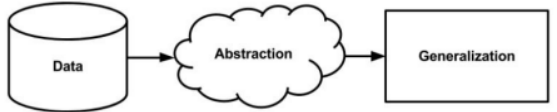
\includegraphics{cap1.png}

}

\caption{Figura 1. Procedimiento de aprendizaje}

\end{Figura 1. Procedimiento de aprendizaje}

El proceso de aprendizaje es más que solo memorizarse parámetro,
preguntas y respuestas. Un ejemplo de esto es el estudio para un examen,
en lugar de tratar de memorizar cada pregunta que se de en un banco, es
mejor ir comprendiendo cada uno de los temas para sacar mejor
calificación. Además, los tres componentes del aprendizaje se encuentran
vinculados entre sí y aunque estos no suceden de manera consiente en los
humanos, por otro lado, en las computadoras se ejecutan de manera
explícita lo que ayuda en su utilización en un futuro.

\hypertarget{abstracciuxf3n-y-representaciuxf3n-del-conocimiento}{%
\subsubsection{Abstracción y representación del
conocimiento}\label{abstracciuxf3n-y-representaciuxf3n-del-conocimiento}}

La representación de datos que entran de manera estructurada y sin
procesar es una de las principales tareas que debe ejecutar un algoritmo
de aprendizaje. Antes de pasar por un procesamiento los datos son solo
unos y ceros en un disco o en la memoria; no llegan a formar ninguna
forma o tienen un significado. Para dar un significado a los mismos
estos deben entrar en un proceso denominado de abstracción. Un ejemplo
de la conexión entre las ideas y la realidad se observa en la famosa
pintura de René Magritte: La traición, que es la imagen que se observa
en la figura dos.

\begin{Figura 2. Pintura de René Magritte}

{\centering 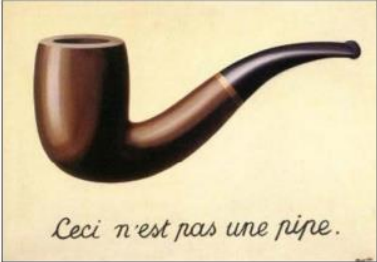
\includegraphics{cap2.png}

}

\caption{Figura 2. Pintura de René Magritte}

\end{Figura 2. Pintura de René Magritte}

La pintura representa una pipa de tabaco con la leyenda Ceci n'est pas
une pipe (``esto no es una pipa''). El punto que Magritte ilustraba es
que una pipa no es realmente una pipa, en donde el autor puede impregnar
la idea de que la imagen representa una tubería, aunque esta no es real,
lo que sugiere que las mentes de los observadores pueden conectar la
imagen de una tubería con la idea de una tubería, que luego puede ser
conectado a una tubería real que podría sostenerse en la mano. Las
conexiones abstraídas como la del ejemplo son una base de la
representación del conocimiento, en donde la formación de estructuras
lógicas ayuda a convertir la información sensorial sin procesar en una
percepción significativa. Existen varios tipos de modelos. Por ejemplo:

• Ecuaciones

• Diagramas como árboles y gráficos

• Reglas lógicas if/else

• Agrupaciones de datos conocidas como clusters La elección del modelo
por lo general la realiza el usuario y no se deja que la máquina elija,
en donde el modelo a elegir debe tener en consideración la tarea de
aprendizaje y el tipo de datos que se analizan. Entrenamiento es el
proceso de ajustar un modelo a un grupo de datos, el ser humano es el
que impone el aprendizaje autónomo a la máquina. El entrenamiento se
encarga de transformar de manera abstracta los datos resumiendo la
información original. Esto se ilustra con el ejemplo del descubrimiento
de la gravedad por Sir Isaac Newton, quien ajustó ecuaciones a datos de
observación para deducir el concepto de gravedad.

\begin{Figura 3. Ilustración de la gravedad}

{\centering 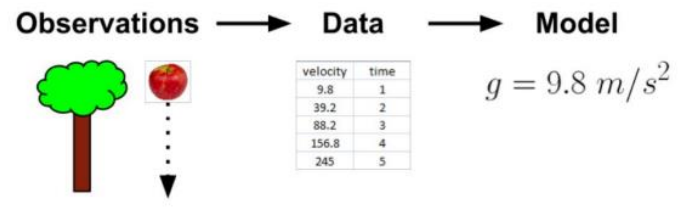
\includegraphics{cap3.png}

}

\caption{Figura 3. Ilustración de la gravedad}

\end{Figura 3. Ilustración de la gravedad}

La mayoría de los modelos no llega a generar teorías que revolucionen el
pensamiento científico, esto puede ayudar para entender las relaciones
entre los datos que no son visibles, por ejemplo, un modelo entrenado
con datos genómicos podría identificar combinaciones de genes
responsables de ciertas enfermedades, o los bancos podrían detectar
patrones de transacciones antes de actividades fraudulentas. Siguiendo
esta idea los psicólogos también podrían identificar nuevas
combinaciones de características que indican trastornos. Los modelos
permiten llegar a dar soluciones de distintas maneras, lo que puede
revelar conexiones previamente desconocidas. La generalización del
aprendizaje se utiliza para tomar acciones futuras, pero esto tiene
varias complicaciones como son las relaciones subyacentes y modelos. Por
ejemplo, la disponibilidad podría explicar por qué la gente tiene más
miedo a volar que a conducir, aunque los accidentes de tráfico son más
comunes, pero menos publicitados. Existe un potencial de las heurísticas
para dar lugar a conclusiones ilógicas, como la falacia del jugador que
puede resultar de la aplicación errónea de la heurística de
representatividad. También se menciona que los algoritmos de aprendizaje
automático pueden estar sesgados si sus heurísticas no son precisas,
como en el caso de un algoritmo que aprendió a identificar caras
basándose en un modelo específico y tiene problemas con rostros que no
se ajustan a ese modelo.

\begin{Figura 4. Proceso}

{\centering 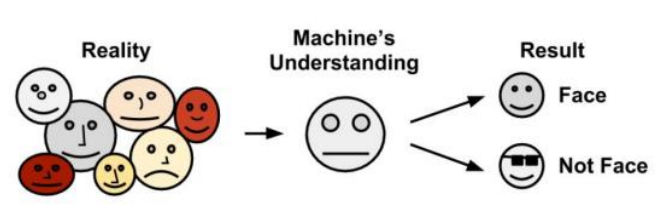
\includegraphics{cap4.png}

}

\caption{Figura 4. Proceso}

\end{Figura 4. Proceso}

\hypertarget{evaluar-el-uxe9xito-del-aprendizaje}{%
\subsubsection{Evaluar el éxito del
aprendizaje}\label{evaluar-el-uxe9xito-del-aprendizaje}}

El sesgo en el aprendizaje automático se convierte en algo importante
para el proceso de generalización, donde cada modelo tiene sus
debilidades y se encuentra sesgado de manera particular. El paso final
en el proceso de generalización es comprobar si funciona el modelo a a
pesar de sus sesgos. Luego se prueba con datos nuevo y se compara con
los valores de los datos del entrenamiento y se generaliza a los nuevos
datos. Un problema para que no se generalicen todos los datos es por el
ruido o variaciones inexplicables en los datos. Los datos ruidosos son
generados de manera aleatoria por:

• Error de medición debido a sensores imprecisos que a veces suman o
restan un poco de la lectura.

• Problemas con los datos de informes, como que los encuestados informen
respuestas aleatorias a las preguntas de la encuesta para terminar más
rápido.

• Errores causados cuando los datos se registran incorrectamente,
incluidos faltantes, nulos, valores truncados, codificados
incorrectamente o corruptos.

Tratar con los ruidos dentro de los datos siempre lleva a realizar
calibraciones dentro de los modelos, donde este se ajusta demasiado a
los datos de entrenamiento, pero ya no generaliza a los nuevos datos,
explicar un ruido lleva a tener errores más complejos y no se identifica
el patrón real.

\hypertarget{pasos-para-aplicar-el-aprendizaje-automuxe1tico-a-sus-datos}{%
\subsubsection{Pasos para aplicar el aprendizaje automático a sus
datos}\label{pasos-para-aplicar-el-aprendizaje-automuxe1tico-a-sus-datos}}

Las tareas de aprendizaje automático se pueden dividir en los siguientes
pasos:

1. Recopilación de datos: ya sea que los datos estén escritos en papel,
registrados en archivos de texto y hojas de cálculo, o almacenados en
una base de datos SQL, deberá recopilarlos en un formato electrónico
adecuado para el análisis. Estos datos servirán como material de
aprendizaje que utiliza un algoritmo para generar conocimiento
procesable

2. Explorar y preparar los datos: la calidad de cualquier aprendizaje
automático mejora del rendimiento del modelo: si se necesita un mejor
rendimiento, se hace necesario utilizar estrategias más avanzadas para
aumentar el rendimiento del modelo. A veces, puede ser necesario cambiar
a un tipo de modelo completamente diferente. Es posible que deba
complementar sus datos con datos adicionales o realizar un trabajo
preparatorio adicional como en el paso dos de este proceso. proyecto se
basa en gran medida en la calidad de los datos que utiliza. Este paso en
el proceso de aprendizaje automático tiende a requerir una gran cantidad
de intervención humana. Una estadística citada a menudo sugiere que el
80 por ciento del esfuerzo en el aprendizaje automático se dedica a los
datos. Gran parte de este tiempo se dedica a aprender más sobre los
datos y sus matices durante una práctica llamada exploración de datos.

3. Entrenamiento de un modelo sobre los datos: Para cuando los datos
hayan sido preparados para análisis, es probable que tenga una idea de
lo que espera aprender de los datos. La tarea específica de aprendizaje
automático informará la selección de un algoritmo apropiado, y el
algoritmo representará los datos en forma de modelo.

4. Evaluación del rendimiento del modelo: debido a que cada modelo de
aprendizaje automático da como resultado una solución sesgada del
problema de aprendizaje, es importante evaluar qué tan bien aprendió el
algoritmo a partir de su experiencia. Según el tipo de modelo utilizado,
es posible que pueda evaluar la precisión del modelo mediante un
conjunto de datos de prueba o que necesite desarrollar medidas de
rendimiento específicas para la aplicación prevista.

5. Mejora del rendimiento del modelo: si se necesita un mejor
rendimiento, se hace necesario utilizar estrategias más avanzadas para
aumentar el rendimiento del modelo. A veces, puede ser necesario cambiar
a un tipo de modelo completamente diferente. Es posible que deba
complementar sus datos con datos adicionales o realizar un trabajo
preparatorio adicional como en el paso dos de este proceso.

Al terminar con estos pasos de manera correcta, y verificando que el
modelo funciona se puede proceder a implementar la tarea prevista. Según
los datos que se estén procesando el modelo se puede utilizar para
proporcionar datos de puntuación para predicciones (posiblemente en
tiempo real), para proyecciones de datos financieros, para generar
información útil para marketing o investigación.

\hypertarget{elegir-un-algoritmo-de-aprendizaje-automuxe1tico}{%
\subsubsection{Elegir un algoritmo de aprendizaje
automático}\label{elegir-un-algoritmo-de-aprendizaje-automuxe1tico}}

Elegir un algoritmo de aprendizaje automático implica tener que realizar
un procedimiento en donde se tengan que hacer coincidir las distintas
características de los datos con los sesgos de los enfoques disponibles.
Esta elección depende del tipo de datos que se manejen y de la tarea
propuesta, a menudo es útil pensar en este proceso mientras recopila,
explora y limpia sus datos.

\hypertarget{pensando-en-los-datos-de-entrada}{%
\subsubsection{Pensando en los datos de
entrada}\label{pensando-en-los-datos-de-entrada}}

Los algoritmos de aprendizaje automático siempre van a necesitar de
datos iniciales, como son ejemplos y características. Los ejemplos son
los conceptos que se va a aprender y estos pueden ser biopsias de
pacientes, etc. En donde la unidad de observación va a describir los que
se mide y sus unidades. Las características por otro lado son atributos
que sirven para aprender el concepto y pueden tener palabras en mensajes
de correo electrónico o datos genómicos de células de biopsia. La
siguiente hoja de cálculo muestra un conjunto de datos en formato de
matriz, lo que significa que cada ejemplo tiene la misma cantidad de
características. En los datos de matriz, cada fila de la hoja de cálculo
es un ejemplo y cada columna es una característica. Aquí, las filas
indican ejemplos de automóviles, mientras que las columnas registran
varias características de los automóviles, como el precio, el
kilometraje, el color y la transmisión. Los datos en formato de matriz
son, con mucho, la forma más común utilizada en el aprendizaje
automático, aunque, como verá en capítulos posteriores, otras formas se
utilizan ocasionalmente en casos especializados.

\begin{Figura 5. Matriz}

{\centering 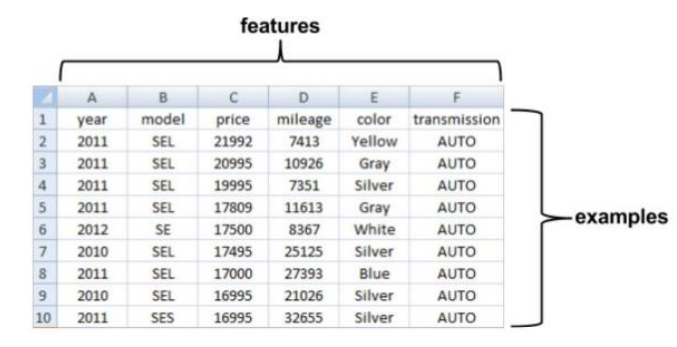
\includegraphics{cap5.png}

}

\caption{Figura 5. Matriz}

\end{Figura 5. Matriz}

A las características que son medidas por números se las conocen como
numéricas. Si se mide un atributo y este está representado por un
conjunto de categorías, se lo llama categórica o nominal. Dentro de este
grupo existe un caso especial al que se le llama ordinal. Algunos
ejemplos de variables ordinales incluyen tallas de ropa como pequeña,
mediana y grande, o una medida de la satisfacción del cliente en una
escala del 1 al 5. Exige dos tipos de modelos utilizados en el análisis
de datos: los modelos predictivos y los modelos descriptivos, los
primeros se utilizan para predecir valores numéricos mediante el ajuste
de modelos de regresión lineal, y los segundos se utilizan para
descubrir patrones en los datos mediante el aprendizaje no supervisado.
La tabla enumera varios tipos de algoritmos, incluyendo árboles de
regresión, agrupación de k-medias, máquinas de vectores de soporte,
redes neuronales, árboles de decisión, reglas de asociación, y
algoritmos de aprendizaje supervisado y no supervisado. La siguiente
tabla enumera los tipos generales de algoritmos de aprendizaje
automático que se tratan en este libro, cada uno de los cuales puede
implementarse de varias maneras.

\begin{Figura 6. Tipos de Algoritmos}

{\centering 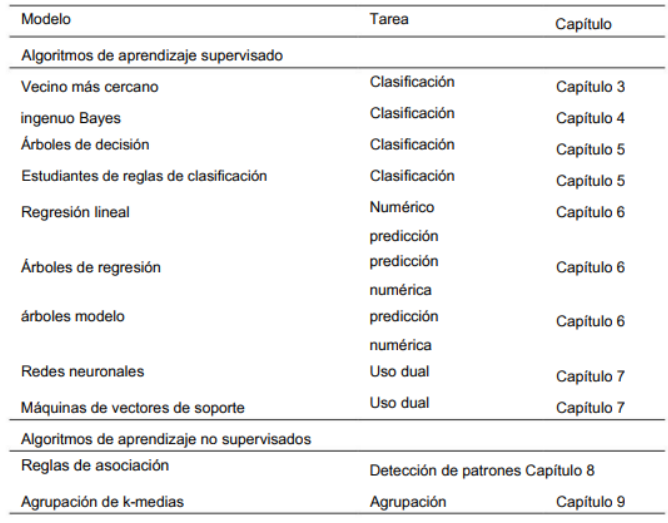
\includegraphics{cap6.png}

}

\caption{Figura 6. Tipos de Algoritmos}

\end{Figura 6. Tipos de Algoritmos}

Para que coincida una tarea con un enfoque de aprendizaje automático, se
necesita identificar el tipo de tarea, su clasificación, predicción
numérica, detección de patrones o agrupación. La elección del algoritmo
dependerá de la tarea y de las fortalezas y debilidades de cada enfoque.
Si es una clasificación lo importantes es como se interpreta el modelo,
para usar R se requiere tener los paquetes que son gratuitos en donde se
encuentran los algoritmos que se necesitan para realizar las distintas
tareas.

\hypertarget{exploraciuxf3n-y-comprensiuxf3n-de-datos}{%
\subsection{\texorpdfstring{\textbf{EXPLORACIÓN Y COMPRENSIÓN DE
DATOS}}{EXPLORACIÓN Y COMPRENSIÓN DE DATOS}}\label{exploraciuxf3n-y-comprensiuxf3n-de-datos}}

Después de que se recopilo los datos, haberlos cargado en estructura de
datos de R, debemos de examinar los datos, explorando sus
características y sus ejemplos, detallando las cosas que hacen que estos
datos sean únicos.

Los datos se llegan a almacenar en formato csv, debemos utilizar
read.csv() para cargar los datos en un marco de datos.

Las preguntas pueden variar entre proyectos, pero estas siempre llegaran
a ser similares.

\hypertarget{explorando-la-estructura-de-los-datos}{%
\subsubsection{Explorando la estructura de los
datos}\label{explorando-la-estructura-de-los-datos}}

Lo primero que debemos tomar en cuenta en una investigación es saber
cómo debemos organizar datos, muchas de las veces la fuente nos
proporcionará un diccionario de datos en el cual también obtendremos un
documento que describe las características de los datos, en el caso de
un coche usado este no viene con la documentación, por lo que se tiene
que crear.

La función str() proporciona~una forma de~mostrar la estructura de un
marco de datos o cualquier estructura de datos R, incluidos vectores y
listas.~Esto se~puede~usar~para crear~un~esquema básico~para~nuestro
diccionario de datos:

El conjunto de datos de usedcars, el número de observaciones se abrevia
con n y se llega a entender que existen 150 ejemplos de automóviles
usados a la venta, se registran 6 variables en los datos que quiere
decir que son 6 características del automóvil, se puede explorar
diferentes detalles adicionales.

Características de color en datos: Después del nombre de variable, chr
nos dice que la función es de tipo carácter, las tres varibales de
indican como int, lo que nos indica el tipo de número entero, este
conjunto solo incluye variables de caracteres y enteros, es posible que
en otros conjuntos como num se encuentren variables numéricas o en tipo
factor los de factores. R no indica una secuencia de primeros valores de
cada característica después de indicarnos su tipo, también nos llega a
mencionar las características como su color: ``Amarillo'', ``Gris'',
``Plata'' y ``Gris''.

\hypertarget{explorando-variables-numuxe9ricas}{%
\subsubsection{Explorando variables
numéricas}\label{explorando-variables-numuxe9ricas}}

Para investigar las variables numéricas en los automóviles usados, se
emplearan conjunto de medidas comunes para describir los valores
conocidos como estadísticas de resumen, la función summary() muestra las
variables estadísticas de resúmenes comunes.

El encabezado de la salida de la función summary() nos puede guiar en
las estadísticas de resumen de datos. En el caso de nuestro ejemplo
anterior los datos serian los numero 2000, 2008, \ldots{} estos nos
indican que la variable se trata del ``año'' de fabricación de los
vehículos ya que estos salieron a la venta recientemente.

También se puede utilizar la función summary () para obtener
estadísticas de resumen de varias variables numéricas al mismo tiempo.

Las seis estadísticas de resumen~proporcionadas por~la función summary()
son herramientas simples pero poderosas para~examinar~datos. Las
estadísticas~resumidas~se pueden dividir en dos tipos: medidas
de~centralidad~y medidas de~dispersión.

La medición de la tendencia central: media y mediana son una clase de
estadística que se suele utilizar para identificar un valor que se
encuentra en el medio de un conjunto de datos, lo más común es que este
ese encuentre ya familiarizado con una medida común del centro que es
conocida como promedio.

El promedio también se conoce como la media, la medida que es conocida
como la suma de todos los valores dividida por el número de valores.

Por ejemplo podemos calcular el grupo de ingreso medio de tres personas
con ingresos de \$35 000, \$45 000 y \$55 000,~ el cual lo podemos
escribir de la siguiente manera.

También podemos encontrar en R la función mean(), que nos ayuda a
calcular la medida de un vector de números.

El promedio que encontramos en este grupo de personas es de \$45.333,33
se puede imaginar esta cantidad como el ingreso que cada persona tendría
si la cantidad total de ingresos se dividiera por igual entre todas las
personas.

Es importante recordar que tanto la media como la mediana son solo dos
de las muchas tendencias centrales disponibles, y cada una tiene sus
propias ventajas y limitaciones. Es importante elegir una medida
apropiada de tendencia central basada en su conjunto de datos y la
pregunta que está tratando de responder.

Un resumen de cinco números es una colección de cinco estadísticas que
representan aproximadamente la dispersión de un conjunto de datos. Hay
cinco estadísticas en la salida de la función summary(). Se escriben en
orden:

\begin{enumerate}
\def\labelenumi{\arabic{enumi}.}
\tightlist
\item
  Minimun (Min.)
\item
  First quartile, or Q1 (1\textsuperscript{st} Qu.)
\item
  Median, or Q2 (Median)
\item
  Third quartile, or Q3 (3\textsuperscript{rd} Qu.)
\item
  Maximum (Max.)
\end{enumerate}

El mínimo y máximo son los valores más extremos que se pueden encontrar
en el conjunto de datos, lo que nos ayuda a encontrar los valores más
pequeños y grandes respectivamente. R nos ayuda proporcionándonos las
funciones min() y max() para calcular estos valores en un vector de
datos.

Encontramos un lapso entre mínimo y máximo se conocen como rango, en R,
la función de este es range() devuelve el valor mínimo como máximo, al
momento que combinamos range() con diff() se permite examinar el tango
de datos con un solo comando.

Los cuartiles primero y tercero, Q1 y Q3, se refieren al valor por
debajo o por encima de una cuarta parte de los valores. Junto con la
mediana (Q2), los cuartiles dividen el conjunto de datos en cuatro
partes, cada una con el mismo número de valores.

Se puede calcular el valor a mano a partir de la salida de resumen para
la variable usedcars\$price calculando 14904 -- 10995=3909,~ R puede
redondear atomáticamente el resumen.

La función quantile() nos da una herramienta robusta que identifica
cuantiles para un conjunto de valores. Un quantile() devuelve el resumen
de cinco números.

Especificamos un parámetro de prueba adicional utilizando un vector que
denota puntos de corte,en los cuales se puede obtener cuantiles
arbitrarios, como percentiles 1 y 99.

La function de secuencia seq() nos ayuda a generar valores espaciados
uniformemente, lo que permite la obtención de otros segmentos de datos
como podemos ver a continuación:

Es una comprension del resumen de cinco números, en el cual se puede
examinar la salida del resumen de automóviles usados.

\hypertarget{visualizaciuxf3n-de-variables-numuxe9ricas}{%
\paragraph{\texorpdfstring{\textbf{Visualización de variables
numéricas}}{Visualización de variables numéricas}}\label{visualizaciuxf3n-de-variables-numuxe9ricas}}

Son de gran utilidad ya que nos ayuda a diagnosticar los problemas de
estos, una visualización común del resumen de cinco números es un
diagrama de caja o un diagrama de caja y bigotes.

El gráfico de la caja muestra el centro y la dispersión de una variable
numérica en un formato que le permite obtener rápidamente una idea del
rango y el sesgo de una variable.

Echemos un vistazo a un diagrama de caja para el precio de un auto usado
y los datos de millaje. Para obtener un diagrama de caja para una
variable, usaremos la función boxplot() . También especificaremos un par
de parámetros adicionales, main e ylab, para agregar un título a la
figura y etiquetar el eje y (el eje vertical), respectivamente. Los
comandos para crear diagramas de caja de precio y kilometraje son.

El diagrama de caja y patillas representa los valores de resumen de
cinco números usando líneas horizontales que forman una imagen en el
medio de cada figura, la mediana está indicada por una línea oscura, que
esta alineada \$13592 en un~ eje vertical.

El minimo y maximo se ilustran con los bigotes que se extienden por
debajo y por encima de la caja; se puede permitir que se extiendan estre
un minimo y un máximo de 1,5 veces que el IQR por debajo de Q1 o por
encima de Q3.

\hypertarget{visualizaciuxf3n-de-variables-numuxe9ricas-histogramas}{%
\paragraph{\texorpdfstring{\textbf{Visualización de variables numéricas:
Histogramas}}{Visualización de variables numéricas: Histogramas}}\label{visualizaciuxf3n-de-variables-numuxe9ricas-histogramas}}

Un histograma es otra forma de representar gráficamente la dispersión de
una variable numérica. Es similar al diagrama de la caja en el sentido
que divide los valores de la variable en un número predefinido de
porciones o contenedores que actúan como contenedores de valores. un
histograma utiliza cualquier número de contenedores de idéntico ancho,
pero permite que los contenedores contengan diferentes cantidades de
valores.

Podemos crear un histograma para el precio de un auto usado y los datos
de kilometraje usando la función hist() .

El histograma se compone de una serie de barras con alturas que indican
el recuento o la frecuencia de los valores que se encuentran dentro de
cada uno de los contenedores de igual tamaño que dividen los valores.

la forma de los dos histogramas es ligeramente diferente. Los precios de
los autos usados \hspace{0pt}\hspace{0pt}parecen estar divididos
equitativamente a ambos lados del medio, mientras que el kilometraje de
los autos todavía varía hacia la derecha. Esta característica se conoce
específicamente como sesgo. desplazamiento a la derecha porque los
valores superiores (derecha) están mucho más dispersos que los valores
inferiores (izquierda). Como se muestra en el siguiente diagrama, los
histogramas de los datos de pendiente aparecen estirados en un lado:

\begin{Figura 7. Histogramas de los datos de pendiente}

{\centering 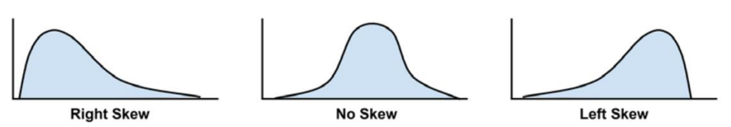
\includegraphics{cap7.png}

}

\caption{Figura 7. Histogramas de los datos de pendiente}

\end{Figura 7. Histogramas de los datos de pendiente}

La capacidad de diagnosticar rápidamente dichos patrones en nuestros
datos es uno de los puntos fuertes del histograma como herramienta de
minería de datos. Esto se vuelve aún más importante cuando comenzamos a
examinar otras distribuciones de datos numéricos.

Comprensión de los números: Distribuciones uniformes y normales
Histogramas, diagramas de caja y estadísticas la gráfica de punto medio
y la distribución proporcionan formas de ver la distribución de los
valores de las variables.

Una distribución uniforme es fácil de detectar con un histograma porque
las barras tienen aproximadamente la misma altura. Cuando se visualiza
con un histograma, puede parecerse al siguiente diagrama:

\begin{Figura 8. Distribución Uniforme}

{\centering 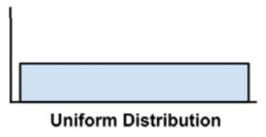
\includegraphics{cap8.png}

}

\caption{Figura 8. Distribución Uniforme}

\end{Figura 8. Distribución Uniforme}

Es importante tener en cuenta que no todos los eventos aleatorios son
uniformes.

Datos de autos usados \hspace{0pt}\hspace{0pt}Claramente esto no es
uniforme ya que algunos valores obviamente son mucho más probables que
otros. De hecho, en un histograma de precios, los valores parecen
aumentar menos cuanto más se encuentran a ambos lados de la banda
central, lo que da como resultado una distribución de datos en forma de
campana. Esta característica es tan común en los datos del mundo real
que es el sello distintivo de la llamada distribución normal.

La curva de campana estereotipada se muestra en el siguiente diagrama:

\begin{Figura 9. Distribución Normal}

{\centering 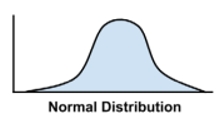
\includegraphics{cap9.png}

}

\caption{Figura 9. Distribución Normal}

\end{Figura 9. Distribución Normal}

\hypertarget{mediciuxf3n-de-la-dispersiuxf3n-varianza-y-desviaciuxf3n-tuxedpica}{%
\paragraph{\texorpdfstring{\textbf{Medición de la dispersión: Varianza y
Desviación
típica}}{Medición de la dispersión: Varianza y Desviación típica}}\label{mediciuxf3n-de-la-dispersiuxf3n-varianza-y-desviaciuxf3n-tuxedpica}}

Para calcular la desviación estándar, primero debemos obtener la
varianza, que se define como el promedio de las diferencias al cuadrado
entre cada valor y el valor medio. En notación matemática, la varianza
de un conjunto de n valores de x se define mediante la siguiente
fórmula. La letra griega mu (similar en apariencia a una m) denota la
media de los valores, y la varianza misma se denota con la letra griega
sigma al cuadrado (similar a ab girada hacia los lados), a continuación,
podemos ver el código para obtener la varianza de los datos:

\begin{Ecuación de la varianza de los datos}

{\centering 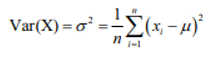
\includegraphics{f1.png}

}

\caption{Ecuación de la varianza de los datos}

\end{Ecuación de la varianza de los datos}

La desviación estándar es la raíz cuadrada de la varianza y se denota
por sigma:

\begin{Desviación estándar}

{\centering 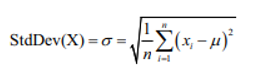
\includegraphics{f2.png}

}

\caption{Desviación estándar}

\end{Desviación estándar}

Para obtener la varianza y la desviación estándar en R se pueden
utilizar las funciones var() y sd() . Por ejemplo, al calcular la
varianza y la desviación estándar de nuestras variables de precio y
millaje, encontramos:

\hypertarget{explorando-variables-categuxf3ricas}{%
\subsubsection{Explorando variables
categóricas}\label{explorando-variables-categuxf3ricas}}

El conjunto de datos de autos usados tenía tres variables categóricas:
modelo, color y transmisión. Debido a que usamos el parámetro
stringsAsFactors = FALSE al cargar los datos, R los ha dejado como
variables de caracteres (chr) en lugar de convertirlos automáticamente
en factores. Además, podríamos considerar tratar el año como categórico;
aunque es como un valor numérico (int), el valor de cada año es una
categoría que podría aplicarse a varios autos.

A diferencia de los datos numéricos, los datos categóricos se examinan
mediante tablas en lugar de estadísticas de resumen. Una tabla que
presenta una única variable categórica se conoce como tabla
unidireccional. La función table() se puede usar para generar tablas
unidireccionales para nuestros datos de autos usados.

Medición de la tendencia central: la moda En términos estadísticos, la
moda de una característica es el valor que se presenta con más
frecuencia. Al igual que la media y la mediana, la moda es otra medida
de tendencia central.

\hypertarget{explorando-relaciones-entre-variables}{%
\subsubsection{Explorando relaciones entre
variables}\label{explorando-relaciones-entre-variables}}

¿Los datos de precios implican que estamos examinando solo automóviles
de clase económica o también hay automóviles de lujo con un alto
kilometraje?

¿Las relaciones entre el modelo y los datos de color brindan información
sobre los tipos de automóviles que estamos examinando?

Este tipo de preguntas se pueden abordar observando las relaciones
bivariados, que consideran la relación entre dos variables. Las
relaciones de más de dos variables se denominan relaciones multivariadas
Empecemos con el caso bivariado.

\hypertarget{visualizaciuxf3n-de-relaciones}{%
\paragraph{\texorpdfstring{\textbf{Visualización de
relaciones:}}{Visualización de relaciones:}}\label{visualizaciuxf3n-de-relaciones}}

~Diagramas de dispersión Un diagrama de dispersión es un diagrama que
visualiza una relación bivariado. Es una figura bidimensional en la que
se dibujan puntos en un plano de coordenadas utilizando los valores de
una característica para proporcionar las coordenadas x horizontales y
los valores de otra característica para proporcionar las coordenadas
verticales y. Los patrones en la ubicación de los puntos revelan
asociaciones subyacentes entre las dos características.

Para responder a nuestra pregunta sobre la relación entre el precio y el
kilometraje, examinaremos un diagrama de dispersión. Usaremos la función
plot() , junto con los parámetros main, xlab e ylab usados en gráficos
anteriores para etiquetar el diagrama.

Comandos para crear diagramas de dispersión.

Usando el diagrama de dispersión, notamos una clara relación entre el
precio de un auto usado y la lectura del odómetro. Para leer el gráfico,
se examina cómo cambian los valores de la variable del eje y a medida
que aumentan los valores del eje x. En este caso, los valores del precio
tienden a ser más bajos a medida que aumentan los valores del
kilometraje, lo que implica que los precios anunciados son más bajos
para los automóviles con mayor kilometraje.

\hypertarget{examen-de-relaciones}{%
\paragraph{\texorpdfstring{\textbf{Examen de
relaciones:}}{Examen de relaciones:}}\label{examen-de-relaciones}}

tabulaciones cruzadas de dos vías Para examinar una relación entre dos
variables nominales, se utiliza una tabulación cruzada de dos vías
(también conocida como tabulación cruzada o tabla de contingencia). Una
tabulación cruzada es similar a un diagrama de dispersión en el sentido
de que le permite examinar cómo los valores de una variable varían según
los valores de otra. El formato es una tabla en la que las filas son los
niveles de una variable mientras que las columnas son los niveles de
otra. Los conteos en cada una de las celdas de la tabla indican el
número de valores que caen en la combinación particular de fila y
columna. Examen de relaciones: tabulaciones cruzadas de dos vías Para
examinar una relación entre dos variables nominales, se utiliza una
tabulación cruzada de dos vías (también conocida como tabulación cruzada
o tabla de contingencia). Una tabulación cruzada es similar a un
diagrama de dispersión en el sentido de que le permite examinar cómo los
valores de una variable varían según los valores de otra. El formato es
una tabla en la que las filas son los niveles de una variable mientras
que las columnas son los niveles de otra. Los conteos en cada una de las
celdas de la tabla indican el número de valores que caen en la
combinación particular de fila y columna.

\hypertarget{comandos-del-ejemplo}{%
\subsection{Comandos del ejemplo}\label{comandos-del-ejemplo}}

Como se explica anteriormente en este apartado pondremos los comandos
del ejemplo:

\begin{Shaded}
\begin{Highlighting}[]
\NormalTok{usedcars }\OtherTok{\textless{}{-}} \FunctionTok{read.csv}\NormalTok{(}\StringTok{"usedcars.csv"}\NormalTok{, }\AttributeTok{stringsAsFactors =} \ConstantTok{FALSE}\NormalTok{)}
\end{Highlighting}
\end{Shaded}

\begin{Shaded}
\begin{Highlighting}[]
\FunctionTok{str}\NormalTok{ (usedcars)}
\end{Highlighting}
\end{Shaded}

\begin{verbatim}
'data.frame':   150 obs. of  6 variables:
 $ year        : int  2011 2011 2011 2011 2012 2010 2011 2010 2011 2010 ...
 $ model       : chr  "SEL" "SEL" "SEL" "SEL" ...
 $ price       : int  21992 20995 19995 17809 17500 17495 17000 16995 16995 16995 ...
 $ mileage     : int  7413 10926 7351 11613 8367 25125 27393 21026 32655 36116 ...
 $ color       : chr  "Yellow" "Gray" "Silver" "Gray" ...
 $ transmission: chr  "AUTO" "AUTO" "AUTO" "AUTO" ...
\end{verbatim}

\begin{Shaded}
\begin{Highlighting}[]
\FunctionTok{summary}\NormalTok{(usedcars}\SpecialCharTok{$}\NormalTok{year)}
\end{Highlighting}
\end{Shaded}

\begin{verbatim}
   Min. 1st Qu.  Median    Mean 3rd Qu.    Max. 
   2000    2008    2009    2009    2010    2012 
\end{verbatim}

\begin{Shaded}
\begin{Highlighting}[]
\FunctionTok{summary}\NormalTok{(usedcars[}\FunctionTok{c}\NormalTok{(}\StringTok{"price"}\NormalTok{, }\StringTok{"mileage"}\NormalTok{)])}
\end{Highlighting}
\end{Shaded}

\begin{verbatim}
     price          mileage      
 Min.   : 3800   Min.   :  4867  
 1st Qu.:10995   1st Qu.: 27200  
 Median :13592   Median : 36385  
 Mean   :12962   Mean   : 44261  
 3rd Qu.:14904   3rd Qu.: 55125  
 Max.   :21992   Max.   :151479  
\end{verbatim}

\begin{Shaded}
\begin{Highlighting}[]
\NormalTok{(}\DecValTok{36000}\SpecialCharTok{+}\DecValTok{44000}\SpecialCharTok{+}\DecValTok{56000}\NormalTok{)}\SpecialCharTok{/}\DecValTok{3}
\end{Highlighting}
\end{Shaded}

\begin{verbatim}
[1] 45333.33
\end{verbatim}

\begin{Shaded}
\begin{Highlighting}[]
\FunctionTok{mean}\NormalTok{(}\FunctionTok{c}\NormalTok{(}\DecValTok{36000}\NormalTok{,}\DecValTok{44000}\NormalTok{,}\DecValTok{56000}\NormalTok{))}
\end{Highlighting}
\end{Shaded}

\begin{verbatim}
[1] 45333.33
\end{verbatim}

\begin{Shaded}
\begin{Highlighting}[]
\FunctionTok{median}\NormalTok{(}\FunctionTok{c}\NormalTok{(}\DecValTok{36000}\NormalTok{,}\DecValTok{44000}\NormalTok{,}\DecValTok{56000}\NormalTok{))}
\end{Highlighting}
\end{Shaded}

\begin{verbatim}
[1] 44000
\end{verbatim}

\begin{Shaded}
\begin{Highlighting}[]
\FunctionTok{range}\NormalTok{(usedcars}\SpecialCharTok{$}\NormalTok{price)}
\end{Highlighting}
\end{Shaded}

\begin{verbatim}
[1]  3800 21992
\end{verbatim}

\begin{Shaded}
\begin{Highlighting}[]
\FunctionTok{diff}\NormalTok{(}\FunctionTok{range}\NormalTok{(usedcars}\SpecialCharTok{$}\NormalTok{price))}
\end{Highlighting}
\end{Shaded}

\begin{verbatim}
[1] 18192
\end{verbatim}

\begin{Shaded}
\begin{Highlighting}[]
\FunctionTok{IQR}\NormalTok{(usedcars}\SpecialCharTok{$}\NormalTok{price)}
\end{Highlighting}
\end{Shaded}

\begin{verbatim}
[1] 3909.5
\end{verbatim}

\begin{Shaded}
\begin{Highlighting}[]
\FunctionTok{quantile}\NormalTok{((usedcars}\SpecialCharTok{$}\NormalTok{price))}
\end{Highlighting}
\end{Shaded}

\begin{verbatim}
     0%     25%     50%     75%    100% 
 3800.0 10995.0 13591.5 14904.5 21992.0 
\end{verbatim}

\begin{Shaded}
\begin{Highlighting}[]
\FunctionTok{quantile}\NormalTok{(usedcars}\SpecialCharTok{$}\NormalTok{price, }\AttributeTok{probs =} \FunctionTok{c}\NormalTok{(}\FloatTok{0.01}\NormalTok{, }\FloatTok{0.99}\NormalTok{))}
\end{Highlighting}
\end{Shaded}

\begin{verbatim}
      1%      99% 
 5428.69 20505.00 
\end{verbatim}

\begin{Shaded}
\begin{Highlighting}[]
\FunctionTok{quantile}\NormalTok{(usedcars}\SpecialCharTok{$}\NormalTok{price, }\FunctionTok{seq}\NormalTok{(}\AttributeTok{from =} \DecValTok{0}\NormalTok{, }\AttributeTok{to =} \DecValTok{1}\NormalTok{, }\AttributeTok{by =} \FloatTok{0.20}\NormalTok{))}
\end{Highlighting}
\end{Shaded}

\begin{verbatim}
     0%     20%     40%     60%     80%    100% 
 3800.0 10759.4 12993.8 13992.0 14999.0 21992.0 
\end{verbatim}

\begin{Shaded}
\begin{Highlighting}[]
 \FunctionTok{boxplot}\NormalTok{(usedcars}\SpecialCharTok{$}\NormalTok{price, }\AttributeTok{main=}\StringTok{"Boxplot of Used Car Prices"}\NormalTok{,}
 \AttributeTok{ylab=}\StringTok{"Price ($)"}\NormalTok{)}
\end{Highlighting}
\end{Shaded}

\begin{figure}[H]

{\centering 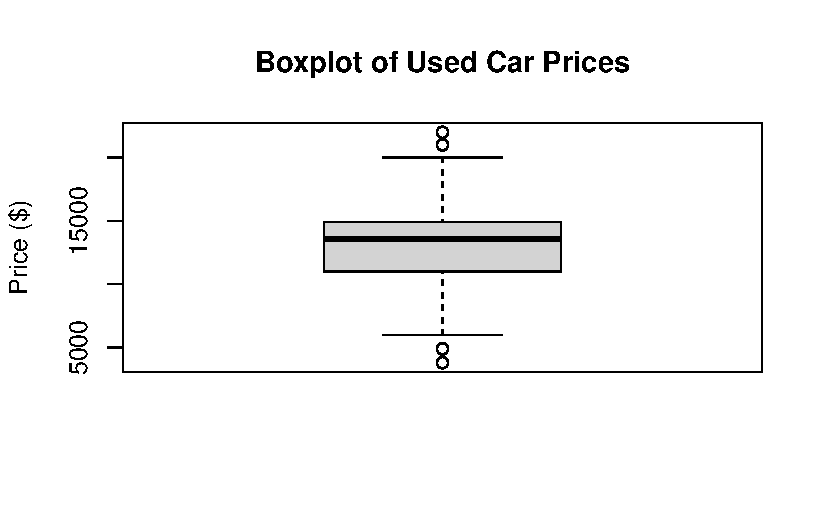
\includegraphics{Unidad_1_files/figure-pdf/unnamed-chunk-14-1.pdf}

}

\end{figure}

\begin{Shaded}
\begin{Highlighting}[]
\FunctionTok{boxplot}\NormalTok{(usedcars}\SpecialCharTok{$}\NormalTok{mileage, }\AttributeTok{main=}\StringTok{"Boxplot of Used Car Mileage"}\NormalTok{,}
 \AttributeTok{ylab=}\StringTok{"Odometer (mi.)"}\NormalTok{)}
\end{Highlighting}
\end{Shaded}

\begin{figure}[H]

{\centering 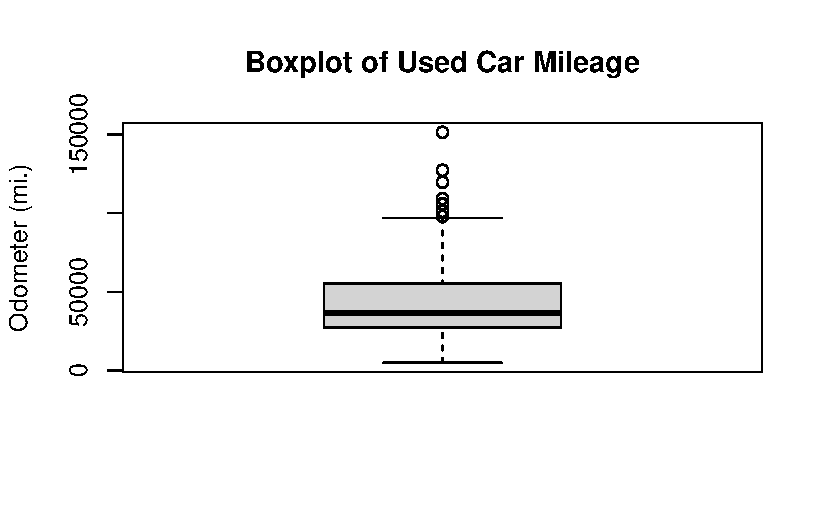
\includegraphics{Unidad_1_files/figure-pdf/unnamed-chunk-14-2.pdf}

}

\end{figure}

\begin{Shaded}
\begin{Highlighting}[]
\FunctionTok{hist}\NormalTok{(usedcars}\SpecialCharTok{$}\NormalTok{price, }\AttributeTok{main =} \StringTok{"Histogram of Used Car Prices"}\NormalTok{,}
 \AttributeTok{xlab =} \StringTok{"Price ($)"}\NormalTok{)}
\end{Highlighting}
\end{Shaded}

\begin{figure}[H]

{\centering 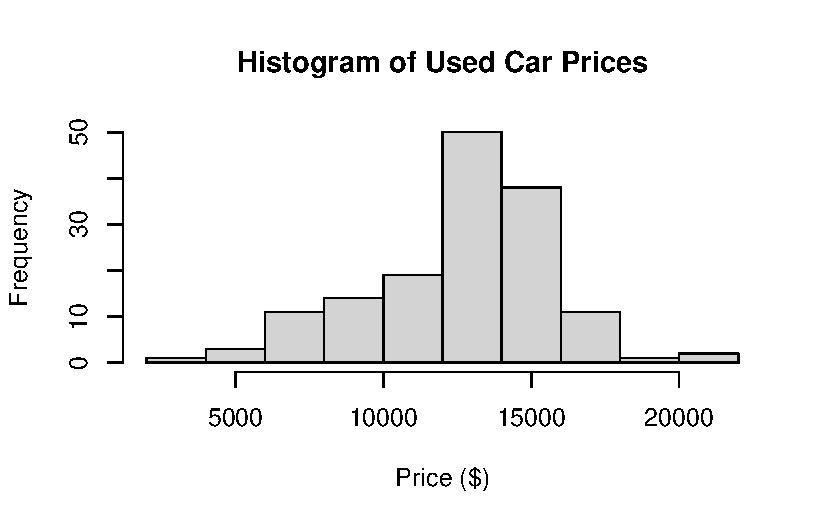
\includegraphics{Unidad_1_files/figure-pdf/unnamed-chunk-15-1.pdf}

}

\end{figure}

\begin{Shaded}
\begin{Highlighting}[]
\FunctionTok{hist}\NormalTok{(usedcars}\SpecialCharTok{$}\NormalTok{mileage, }\AttributeTok{main =} \StringTok{"Histogram of Used Car Mileage"}\NormalTok{,}
 \AttributeTok{xlab =} \StringTok{"Odometer (mi.)"}\NormalTok{)}
\end{Highlighting}
\end{Shaded}

\begin{figure}[H]

{\centering 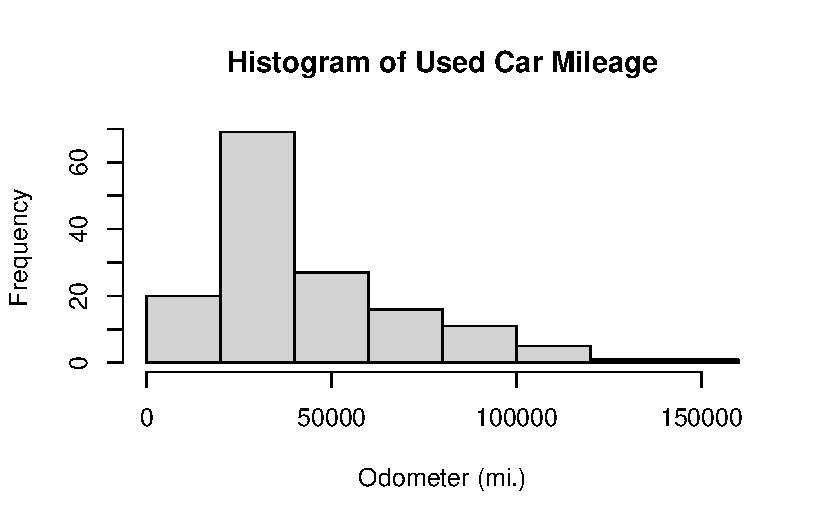
\includegraphics{Unidad_1_files/figure-pdf/unnamed-chunk-15-2.pdf}

}

\end{figure}

\begin{Shaded}
\begin{Highlighting}[]
\FunctionTok{var}\NormalTok{(usedcars}\SpecialCharTok{$}\NormalTok{price)}
\end{Highlighting}
\end{Shaded}

\begin{verbatim}
[1] 9749892
\end{verbatim}

\begin{Shaded}
\begin{Highlighting}[]
\FunctionTok{sd}\NormalTok{(usedcars}\SpecialCharTok{$}\NormalTok{price)}
\end{Highlighting}
\end{Shaded}

\begin{verbatim}
[1] 3122.482
\end{verbatim}

\begin{Shaded}
\begin{Highlighting}[]
\FunctionTok{var}\NormalTok{(usedcars}\SpecialCharTok{$}\NormalTok{mileage)}
\end{Highlighting}
\end{Shaded}

\begin{verbatim}
[1] 728033954
\end{verbatim}

\begin{Shaded}
\begin{Highlighting}[]
\FunctionTok{sd}\NormalTok{(usedcars}\SpecialCharTok{$}\NormalTok{mileage)}
\end{Highlighting}
\end{Shaded}

\begin{verbatim}
[1] 26982.1
\end{verbatim}

\begin{Shaded}
\begin{Highlighting}[]
 \FunctionTok{table}\NormalTok{(usedcars}\SpecialCharTok{$}\NormalTok{year)}
\end{Highlighting}
\end{Shaded}

\begin{verbatim}

2000 2001 2002 2003 2004 2005 2006 2007 2008 2009 2010 2011 2012 
   3    1    1    1    3    2    6   11   14   42   49   16    1 
\end{verbatim}

\begin{Shaded}
\begin{Highlighting}[]
 \FunctionTok{table}\NormalTok{(usedcars}\SpecialCharTok{$}\NormalTok{model)}
\end{Highlighting}
\end{Shaded}

\begin{verbatim}

 SE SEL SES 
 78  23  49 
\end{verbatim}

\begin{Shaded}
\begin{Highlighting}[]
\FunctionTok{table}\NormalTok{(usedcars}\SpecialCharTok{$}\NormalTok{color)}
\end{Highlighting}
\end{Shaded}

\begin{verbatim}

 Black   Blue   Gold   Gray  Green    Red Silver  White Yellow 
    35     17      1     16      5     25     32     16      3 
\end{verbatim}

\begin{Shaded}
\begin{Highlighting}[]
\NormalTok{model\_table }\OtherTok{\textless{}{-}} \FunctionTok{table}\NormalTok{(usedcars}\SpecialCharTok{$}\NormalTok{model)}
\FunctionTok{prop.table}\NormalTok{(model\_table)}
\end{Highlighting}
\end{Shaded}

\begin{verbatim}

       SE       SEL       SES 
0.5200000 0.1533333 0.3266667 
\end{verbatim}

\begin{Shaded}
\begin{Highlighting}[]
\NormalTok{color\_table }\OtherTok{\textless{}{-}} \FunctionTok{table}\NormalTok{(usedcars}\SpecialCharTok{$}\NormalTok{color)}
\NormalTok{color\_pct }\OtherTok{\textless{}{-}} \FunctionTok{prop.table}\NormalTok{(color\_table) }\SpecialCharTok{*} \DecValTok{100}
\FunctionTok{round}\NormalTok{(color\_pct, }\AttributeTok{digits =} \DecValTok{1}\NormalTok{)}
\end{Highlighting}
\end{Shaded}

\begin{verbatim}

 Black   Blue   Gold   Gray  Green    Red Silver  White Yellow 
  23.3   11.3    0.7   10.7    3.3   16.7   21.3   10.7    2.0 
\end{verbatim}

\begin{Shaded}
\begin{Highlighting}[]
\FunctionTok{plot}\NormalTok{(}\AttributeTok{x =}\NormalTok{ usedcars}\SpecialCharTok{$}\NormalTok{mileage, }\AttributeTok{y =}\NormalTok{ usedcars}\SpecialCharTok{$}\NormalTok{price,}
 \AttributeTok{main =} \StringTok{"Scatterplot of Price vs. Mileage"}\NormalTok{,}
 \AttributeTok{xlab =} \StringTok{"Used Car Odometer (mi.)"}\NormalTok{,}
 \AttributeTok{ylab =} \StringTok{"Used Car Price ($)"}\NormalTok{)}
\end{Highlighting}
\end{Shaded}

\begin{figure}[H]

{\centering 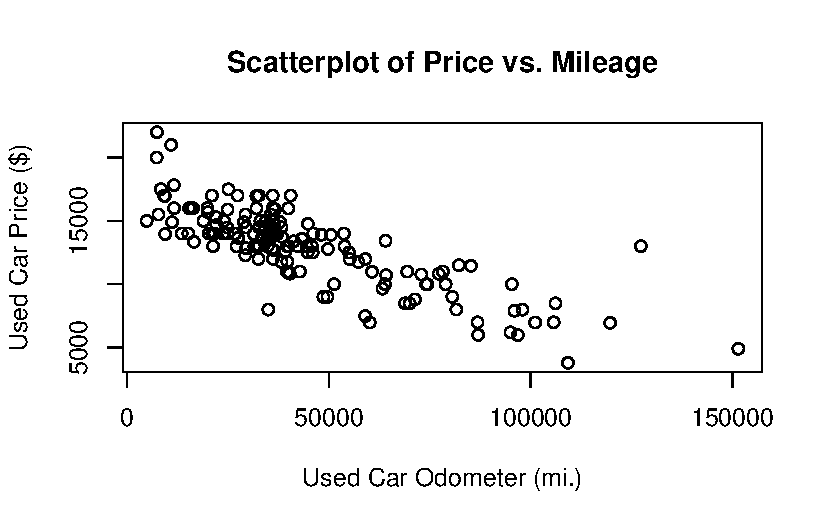
\includegraphics{Unidad_1_files/figure-pdf/unnamed-chunk-25-1.pdf}

}

\end{figure}

Para esta parte del ejemplo se debe instalar la librería gmodels para
los cual se puede utilizar el comando: (install.packages(``gmodels'')).

\begin{Shaded}
\begin{Highlighting}[]
\FunctionTok{library}\NormalTok{(gmodels)}
\end{Highlighting}
\end{Shaded}

\begin{Shaded}
\begin{Highlighting}[]
\NormalTok{ usedcars}\SpecialCharTok{$}\NormalTok{conservative }\OtherTok{\textless{}{-}}
\NormalTok{ usedcars}\SpecialCharTok{$}\NormalTok{color }\SpecialCharTok{\%in\%} \FunctionTok{c}\NormalTok{(}\StringTok{"Black"}\NormalTok{, }\StringTok{"Gray"}\NormalTok{, }\StringTok{"Silver"}\NormalTok{, }\StringTok{"White"}\NormalTok{)}
\end{Highlighting}
\end{Shaded}

\begin{Shaded}
\begin{Highlighting}[]
 \FunctionTok{table}\NormalTok{(usedcars}\SpecialCharTok{$}\NormalTok{conservative)}
\end{Highlighting}
\end{Shaded}

\begin{verbatim}

FALSE  TRUE 
   51    99 
\end{verbatim}

\begin{Shaded}
\begin{Highlighting}[]
\FunctionTok{CrossTable}\NormalTok{(}\AttributeTok{x =}\NormalTok{ usedcars}\SpecialCharTok{$}\NormalTok{model, }\AttributeTok{y =}\NormalTok{ usedcars}\SpecialCharTok{$}\NormalTok{conservative)}
\end{Highlighting}
\end{Shaded}

\begin{verbatim}

 
   Cell Contents
|-------------------------|
|                       N |
| Chi-square contribution |
|           N / Row Total |
|           N / Col Total |
|         N / Table Total |
|-------------------------|

 
Total Observations in Table:  150 

 
               | usedcars$conservative 
usedcars$model |     FALSE |      TRUE | Row Total | 
---------------|-----------|-----------|-----------|
            SE |        27 |        51 |        78 | 
               |     0.009 |     0.004 |           | 
               |     0.346 |     0.654 |     0.520 | 
               |     0.529 |     0.515 |           | 
               |     0.180 |     0.340 |           | 
---------------|-----------|-----------|-----------|
           SEL |         7 |        16 |        23 | 
               |     0.086 |     0.044 |           | 
               |     0.304 |     0.696 |     0.153 | 
               |     0.137 |     0.162 |           | 
               |     0.047 |     0.107 |           | 
---------------|-----------|-----------|-----------|
           SES |        17 |        32 |        49 | 
               |     0.007 |     0.004 |           | 
               |     0.347 |     0.653 |     0.327 | 
               |     0.333 |     0.323 |           | 
               |     0.113 |     0.213 |           | 
---------------|-----------|-----------|-----------|
  Column Total |        51 |        99 |       150 | 
               |     0.340 |     0.660 |           | 
---------------|-----------|-----------|-----------|

 
\end{verbatim}



\end{document}
